\documentclass[11pt]{article}

\usepackage[margin=1in,letterpaper]{geometry}
\usepackage{amsmath,bm}
\usepackage{siunitx}
\usepackage{enumitem}
%\usepackage{times}
\usepackage{graphicx}
\usepackage{tikz}
\usepackage{mathpazo}
%\usepackage[scaled]{helvet}
%\usepackage{xcolor,colortbl}
%\usepackage{hyperref}
%\usepackage{cancel}

\setlength{\parindent}{0pt}
%\setlength{\parskip}{1em}

%\usetikzlibrary{decorations.pathmorphing,patterns}

\sisetup{
  detect-all,
  number-math-rm=\mathnormal,
  per-mode=symbol
}

\title{Kepler's Laws of Planetary Motion}
\author{Dr.\ Timothy M.\ Leung}
\date{\today}

\newcommand{\pic}[2]{
  \includegraphics[width=#1\textwidth]{#2}
}
\newcommand{\mb}[1]{
  \ensuremath\mathbf{#1}
}
\newcommand{\eq}[2]{
  \vspace{#1}{\Large
    \begin{displaymath}
      #2
    \end{displaymath}
  }
}

\begin{document}
\maketitle

%Kepler's laws describe the motion of objects in the presence of a central
%inverse square force. For simplicity, we'll consider the motion of the planets
%in our solar system around the Sun, with gravity as the central force. Among
%other things, Kepler's laws allow one to predict the position and velocity of
%the planets at any given time, the time for a satellite to collapse into the
%surface of a planet, and the period of a planet's orbit as a function of its
%orbits' geometry.
%
Although the laws were originally obtained by Kepler after careful analysis of
empirical data from his teacher Tycho Brahe, the complete mathematical
understanding was missing until Newton derived each law as pieces of his
orbital mechanics. In his footsteps we will obtain each law in turn, as we
consider the orbit of a planet in the gravity of a massive star. In modern
form, \textbf{Kepler's laws of planetary motion} state that:
\begin{enumerate}[leftmargin=18pt]
\item A planet moves around the Sun in an elliptical path with the Sun as one
  of the focii.
\item The line segment joining a planet and the Sun sweeps out equal areas
  during equal intervals of time
\item The square of the orbital time period of a planet is proportional to the
  cube of the semi-major axis of its orbit, i.e.\ $T^2\propto r^3$.
\end{enumerate}

Two properties of gravity are crucial to understanding of orbital mechanics.
These two properties are true regardless of the shape of the orbit, and even
whether an object is in orbit or not:
\begin{enumerate}[leftmargin=18pt]
\item Gravity is a \emph{conservative} force, in that
  \begin{itemize}[leftmargin=15pt]
  \item Assuming that minor collisions with space dust and other methods of
    energy dissipation are negligible, then the mechanical energy
    $E=K+U_g$ is conserved.
  \item Work done \emph{by} gravity converts gravitational potential energy
    $U_g$ into kinetic energy $K$, while work \emph{against} gravity converts
    $K$ into $U_g$.
  \end{itemize}
\item Gravity is a \emph{central} force, in that
  \begin{itemize}[leftmargin=15pt]
  \item Because gravitational force $\mb{F}_g$ is always in the $-\hat{\mb{r}}$
    direction, i.e.\ $\mb{F}\times\mb{r}=\mb{0}$,  therefore gravity does not
    generate any torque
  \item Angular momentum $\mb{L}$ is constant as a result
  \item The motion of the planet is confined to a two-dimensional plane
  \end{itemize}
\end{enumerate}
For the purpose of the analysis, we also assume that the Sun's mass $M_\odot$
is very large compared to any other object in the solar system, and  its motion
is essentially unaffected by the gravity from the planets.


\section{Second law: Equal area in equal time}
The second law of planetary motion is the easiest to proof using concepts in
rotational motion.
\begin{figure}[ht]
  \begin{center}
    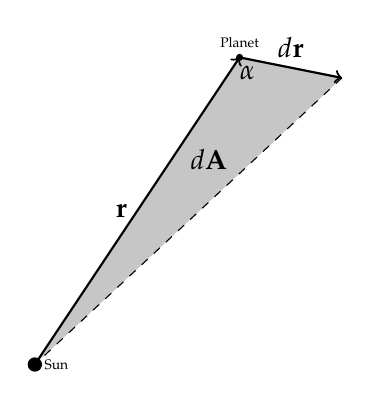
\begin{tikzpicture}[scale=1.3]
      \fill[gray!45](0,0)--(2,3)--(3,2.8)--cycle;
      \node at (1.7,2) {$d\mb{A}$};
      \draw[->,thick](0,0)--(2,3)
      node[midway,left]{$\mb{r}$} node[pos=.95,right]{$\alpha$};
      \draw[->,thick](2,3)--(3,2.8) node[midway,above]{$d\mb{r}$};
      \draw[dashed](3,2.8)--(0,0);
      \fill[black](0,0) circle(.07) node[right]{\tiny\textrm{Sun}};
      \fill[black](2,3) circle(.035)node[above]{\tiny\textrm{Planet}};
    \end{tikzpicture}
    \end{center}
  \caption{Infinitesimal area swept by a planet as it moves in orbit.}
  \label{fig:dA}
\end{figure}
The infinitesimal area $d\mb{A}$ (Figure \ref{fig:dA}) swept out by a planet as
it moves in orbit by an infinitesimal amount $d\mb{r}$ can be computed by the
area of the triangle:
\begin{equation}
  dA=\frac{1}{2}rdr\sin\alpha
\end{equation}
or in vector form:
\begin{equation}
  d\mb{A}=\frac{1}{2}\mb{r}\times d\mb{r}
\end{equation}
The direction of $d\mb{A}$, in this case, points into the page. The time
derivative of the area is called the \textbf{areal velocity}, which literally
means how quickly the area is changing:
\begin{equation}
  \frac{d\mb{A}}{dt}
  =\frac{1}{2}\mb{r}\times\frac{d\mb{r}}{dt}
  =\frac{1}{2}\mb{r}\times\mb{v}
\end{equation}
We can express $\mb{r}\times\mb{v}$ in terms of angular momentum,
$\mb{L}=m(\mb{r}\times\mb{v})$. Since gravity is a central force, angular
momentum is a constant, i.e:
\begin{equation}
  \boxed{\frac{d\mb{A}}{dt}
    =\frac{1}{2}(\mb{r}\times\mb{v})=\frac{\mb{L}}{2m}=
    \text{constant}
  }
  \label{constant}
\end{equation}
as predicted by Kepler's second law. The rate a planet sweeps out the area in
orbit is its angular momentum around the sun, divided by twice its mass.


%If we had instead multiplied \ddot{x} 
%x
%¨
%  by \sin\thetasinθ, \ddot{y} 
%y
%¨
%​	
%  by \cos\thetacosθ, and subtract the equations, we would find
%
%r\ddot{\theta} + 2\dot{r}\dot{\theta} = 0.
%r 
%θ
%¨
% +2 
%r
%˙
%  
%θ
%˙
% =0.
%
%If we multiply this equation by rr, we find r^2\ddot{\theta} + 2r\dot{r}\dot{\theta}=0r 
%2
%  
%θ
%¨
% +2r 
%r
%˙
%  
%θ
%˙
% =0. However, this is just the time derivative of r^2\dot{\theta}r 
%2
%  
%θ
%˙
% , and thus we have shown
%
%\frac{d}{dt}r^2\dot{\theta} = 0.
%dt
%d
%​	
% r 
%2
%  
%θ
%˙
% =0.
%
%But mr^2\dot{\theta}mr 
%2
%  
%θ
%˙
%  is the angular momentum of the planet. Thus, the angular momentum of the planet is conserved.
%
%If we integrate this equation with respect to time, we find that mr^2\dot{\theta} = L,mr 
%2
%  
%θ
%˙
% =L, where L is a constant. Integrating once more in time, we find
%
%\begin{align*}
%  \int L dt &= m\int r^2 \frac{d\theta}{dt} dt\\ &= m\int_{\theta_i}^{\theta_f} r^2 d\theta.
%\end{align*}
% 
%
%The integral \frac12 \int r^2 d\theta 
%2
%1
%​	
% ∫r 
%2
% dθ is the area swept out by the radial vector from the Sun to the planet in moving from \theta_iθ 
%i
%​	
%  to \theta_fθ 
%f
%​	
% . However, the result is independent of \theta_iθ 
%i
%​	
%  and \theta_fθ 
%f
%​	
% , but it only depends on tt since the angular momentum is constant.
%
%Thus, we have derived Kepler's second law, i.e. segments of orbits sweep out equal areas in equal intervals of time:
%
%\boxed{\displaystyle\frac12\int_{\text{any path}} r^2 d\theta = \frac{Lt}{2m}}.
%2
%1
%​	
% ∫ 
%any path
%​	
% r 
%2
% dθ= 
%2m
%Lt
%​	
% 
%​	
% .
%The speed of a certain planet at the perihelion is v_pv 
%p
%​	
%  and, at this position, the distance of the sun from the planet is r_pr 
%p
%​	
% . Relate \{r_p,v_p\}{r 
%p
%​	
% ,v 
%p
%​	
% } to the corresponding quantities at the aphelion \{r_a,v_a\}{r 
%a
%​	
% ,v 
%a
%​	
% }.
%
%The magnitude of the angular momentum at perihelion is L_p=m_pr_pv_pL 
%p
%​	
% =m 
%p
%​	
% r 
%p
%​	
% v 
%p
%​	
%  because r_pr 
%p
%​	
%  and v_pv 
%p
%​	
%  are mutually perpendicular. Similarly, L_a=m_pr_av_aL 
%a
%​	
% =m 
%p
%​	
% r 
%a
%​	
% v 
%a
%​	
% . Using the conservation of angular momentum,
%
%m_pr_pv_p=m_pr_av_a\Rightarrow r_pv_p=r_av_a \Rightarrow \dfrac{v_p}{v_a} = \dfrac{r_a}{r_p}.

\section{First Law: The Law of Ellipses}
In order to proof Kepler's first law, we must show that all orbital motion must
agree with the equations of an ellipse, which is in the form:
\begin{equation}
  r=\frac{a(1-e^2)}{1+e\cos\theta}
  \quad\textnormal{\normalsize where}\quad
  0\leq e < 1
\end{equation}
where $e$ is called the eccentricity of the ellipse.
\begin{equation}
  \frac{d^2r}{dt^2} - r\frac{d\omega}{dt}^2 = -GM\frac{1}{r^2}
  \label{differential}
\end{equation}


\begin{figure}[!ht]
  \centering
  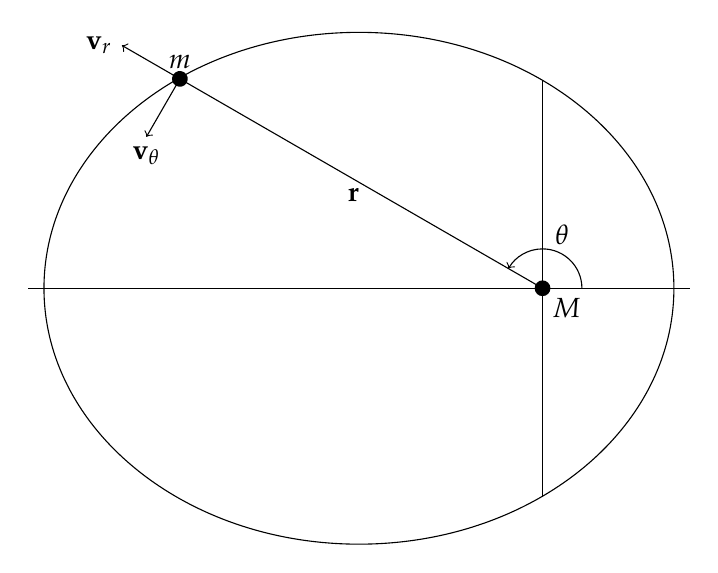
\begin{tikzpicture}
    \def\a{4} % semi-major axis
    \def\b{3.25} % semi-minor axis
    \def\angle{150} % angle
    \draw (0,0) ellipse ({\a} and {\b});% Draw the ellipse
    \draw ({sqrt(\a*\a-\b*\b)},-2.65)--({sqrt(\a*\a-\b*\b)},2.65);
    \draw (-\a-.2,0)--(\a+.2,0);
    \fill[black]({sqrt(\a*\a-\b*\b)},0) circle(.1) node[below right]{$M$};
    \begin{scope}[rotate around={\angle:({sqrt(\a*\a-\b*\b)},0)}]
      \draw[->]({sqrt(\a*\a-\b*\b)},0)--(8.5,0)
      node[pos=.45,below]{$\mb{r}$} node[pos=1,left]{$\mb{v}_r$};
      \draw[->](7.65,0)--(7.65,.85) node[below]{$\mb{v}_\theta$};
      \fill (7.65,0) circle(.1) node[above]{$m$};
    \end{scope}
    \draw[->]({sqrt(\a*\a-\b*\b)+.5},0) arc(0:\angle:.5)
    node[pos=.4,above]{$\theta$};
%      \draw[<->]({sqrt(\a*\a-\b*\b)-.2},0)--({sqrt(\a*\a-\b*\b)-.2},-2.65)
%      node[midway,left]{\tiny$r_0$};
  \end{tikzpicture}
  \caption{Elliptical orbit of a small mass $m$ around a large mass $M$.}
  \label{eorbit}
\end{figure}


As shown in Fig.~\ref{eorbit}, there are two components of velocity when a
planet orbits a star:
\begin{itemize}
\item\textbf{Angular velocity} $\mb{v}_\theta$. The presence of $\mb{v}_\theta$
  means a centripetal acceleration toward $M$:
  \begin{equation}
    a=-r\omega^2\hat{\mb{r}}
  \end{equation}
\item\textbf{Radial velocity} $\mb{v}_r$. If this velocity changes with time
  (which is the case for elliptical orbits but not circular orbits), then there
  is an acceleration, also in the radial direction:
  \begin{equation}
    a=\frac{dr}{dt}\hat{\mb{r}}
  \end{equation}
\end{itemize}
Both components of acceleration are due entirely to gravitational force.
Applying Newton's second law of motion gives the differential equation:
\begin{equation}
  \frac{d^2r}{dt^2}-r\omega^2=-\frac{GM}{r^2}
  \label{ode1}
\end{equation}
The ($+$) direction is radially outward from $M$. In the circular motion case,
where $d^2r/dt^2=0$, we are left with only the centripetal force.

The differential equation, in its current form, is difficult to solve, and the
equation for an ellipse depends on $\theta$ but not on $t$. However, the
differential equation is easier to solve by making a variable substitution that
may not be immediately obvious, by introducing a new variable $u$ which is
the inverse of the radius $r$:
\begin{equation}
  u=\frac{1}{r}
\end{equation}
We can then use the fact that angular momentum $L$ is constant to relate
derivatives in time $t$ to derivatives in angle $\theta$:
\begin{equation}
  L=mr^2\frac{d\theta}{dt}=\frac{m}{u^2}\frac{d\theta}{dt}
  \quad\longrightarrow\quad
  \frac{d}{d\theta}=\frac{Lu^2}{m}\frac{d}{dt}
\end{equation}
The derivatives $\dot{r}$ and $\ddot{r}$ can now be expressed in terms of
derivatives with respect to $\theta$ instead of time:
\begin{align}
  \frac{dr}{dt} &=\frac{d}{dt}\left(\frac{1}{u}\right)
  =-\frac{1}{u}\frac{du}{dt}\\
  &=-\frac{L}{m}\frac{du}{d\theta}\\
  &= -u^{-2}\frac{du}{d\theta} \frac{Lu^2}{m} \\
  &= -\frac{L}{m}\frac{du}{d\theta}
\end{align}
Repeating the same process for the second derivative, we have
\begin{align}
  \frac{d^2r}{dt^2} &= \frac{d}{dt}\left(-\frac{L}{m}\frac{du}{d\theta}\right)\\
  &= -\frac{L}{m} \frac{d}{d\theta}\frac{du}{d\theta} \\
  &= -\left(\frac{L^2u^2}{m^2}\right)\frac{d^2u}{d\theta^2}
\end{align}
With this identity in hand, our original differential equation
(Eq.\ \ref{differential}) becomes
\begin{equation}
  -\left(\frac{L^2u^2}{m^2}\right)\frac{d^2u}{d\theta^2} - \left(\frac{L}{m}\right)^2u^3 = -GMu^2
\end{equation}
which can be simplified to:
\begin{equation}
  \frac{d^2u}{d\theta^2} + u = \frac{GMm^2}{L^2}
  \label{newdiff}
\end{equation}

Anyone experienced with calculus should immediately recognize that
Eq.\ \ref{newdiff} is a second-order ordinary differential equation with
constant coefficients and a constant forcing function. The solution to this
type of equation is in the form
\begin{equation}
  u =A\cos\theta + \frac{GMm^2}{L^2}
\end{equation}
where the coefficient $A$ is determined by initial conditions. Solving for
$r=1/u$, we have
\begin{equation}
  r(\theta)= \frac{1}{A\cos\theta+ \frac{GMm^2}{L^2}}
  =\left(\frac{L^2}{GMm^2}\right)\frac{1}{1+e\cos\theta}
\end{equation}
where $e$ is a constant:
\begin{equation}
  e=\dfrac{AL^2}{GMm^2}
\end{equation}
From this form of $r$, it is clear that the maximum and a minumum values of
$r$, in fact represent the \emph{aphelion} and \emph{perihelion} of the
ellipes (points of furthest and closest distance to the focys):
\begin{equation}
  r_{\textrm{max}}=\left(\frac{L^2}{GMm^2}\right)\frac{1}{1-e}
  \quad\quad
  r_{\textrm{min}}=\left(\frac{L^2}{GMm^2}\right)\frac{1}{1+e}
\end{equation}
This the semi-major axis $r$ is the average of the two values:
\begin{equation}
  a=\dfrac12\left(r_\text{min} + r_\text{max}\right)=
  \left(\frac{L^2}{GMm^2}\right)\frac{1}{1-e^2}
  \label{semimajor}
\end{equation}
More importantly, Eq.\ \ref{semimajor} allows us to relate the eccentricity
$e$ and the semi-major axis $a$ to the numerator in the $r$ expression:
\begin{equation}
  a(1-e^2)=\frac{L^2}{GMm^2}
  \label{eq:numerator}
\end{equation}
We see that the orbit is given by an ellipse as Kepler found from Brahe's
dataset. Moreover, since $r_\mathrm{min}$ and $r_\mathrm{max}$ are distances from
the Sun, we see that the Sun is at one focus of the orbit. Thus, we have
derived Kepler's first law.

%$r\sim\left(1+e\cos\theta\right)^{-1}$ is the general form of an ellipse in
%polar coordinates, with the origin placed at a focus. In the study of ellipses,
%the parameter ee is often called the eccentricity. When the eccentricity of a
%planet's orbit is zero, the orbit is perfectly circular. As $e$ approaches one,
%the orbit is stretched out into more elongated elliptical trajectories. To
%demonstrate this feature, we plot the orbit below for several values of the
%eccentricity, $e$.
%
%
%\text{Plot of the orbit for increasing eccentricity}, e
%Plot of the orbit for increasing eccentricity,e
%What happens if e \geq 1e≥1?

\section{Third law: Period of motion}
\begin{figure}
  \centering
  \pic{.5}{../kep8.png}
  \caption{The pl}
  \label{3rdlaw}
\end{figure}
The total area $A$ swept by the planet through one orbital period is the areal
velocity (which is constant, as shown in Eq.\ \ref{constant}) integrated by
time, from $t=0$ to $T$, the orbital period of the planet:
\begin{equation}
  A=\int dA=\int_0^T\frac{dA}{dt}dt=\frac{L}{2m}\int_0^Tdt=\frac{L}{2m}T
  \label{A1}
\end{equation}
From proofing Kepler's first law in the previous section, we know that this
area is an ellipse, given by the equation:
\begin{equation}
  A=\pi ab=\pi a^2\sqrt{1-e^2}
  \label{A2}
\end{equation}
where $a$ is the semi-major axis, $b=a\sqrt{1-e^2}$ is the semi-minor axis.
Equating the expressions for area in Eq.\ \ref{A1} and Eq.\ \ref{A2}, then
squaring both sides, give this expression:
\begin{equation}
  T^2=\frac{m^2}{L^2}4\pi^2a^4(1-e^2)
  \label{eq:almost}
\end{equation}
Substituting Eq. \ref{eq:numerator}, shown below for reference:
\begin{displaymath}
  a(1-e^2)=\frac{L^2}{GMm^2}
\end{displaymath}
into Eq.\ \ref{eq:almost} above, and after some simple algebra, we arrive at
this expression:
\begin{equation}
  \boxed{T^2=\left[\frac{4\pi^2}{GM}\right] a^3}
\end{equation}
which is Kepler's third law. Note that this law holds for all elliptical
orbits, regardless of their eccentricities.
\end{document}
